\documentclass[a4paper,12pt]{article}

\usepackage[utf8]{inputenc}
\usepackage[T1]{fontenc}
\usepackage{amsmath}
\usepackage{booktabs}
\usepackage{graphicx}
\usepackage{geometry}
\geometry{margin=2.5cm}
\usepackage{xcolor}
\usepackage{listings}
\usepackage{hyperref}
\hypersetup{colorlinks=true, linkcolor=blue!50!black, urlcolor=blue!50!black}
\renewcommand{\tablename}{Tabela}
\renewcommand{\figurename}{Figura}
\renewcommand{\lstlistingname}{Código}

\definecolor{codebg}{RGB}{247,247,247}
\definecolor{codekw}{RGB}{0,0,180}
\definecolor{codecomment}{RGB}{0,128,0}
\definecolor{codestring}{RGB}{163,21,21}
\definecolor{framecolor}{RGB}{200,200,200}

\lstdefinestyle{cstyle}{
    language=C,
    backgroundcolor=\color{codebg},
    basicstyle=\ttfamily\footnotesize,
    keywordstyle=\color{codekw}\bfseries,
    commentstyle=\color{codecomment}\itshape,
    stringstyle=\color{codestring},
    numberstyle=\tiny\color{gray},
    numbers=left,
    numbersep=6pt,
    frame=single,
    rulecolor=\color{framecolor},
    breaklines=true,
    breakatwhitespace=false,
    showstringspaces=false,
    tabsize=4,
    captionpos=b,
    columns=flexible,
    morekeywords={size_t},
    extendedchars=true,
    literate=
        {á}{{\'a}}1 {à}{{\`a}}1 {â}{{\^a}}1 {ã}{{\~a}}1
        {é}{{\'e}}1 {ê}{{\^e}}1 {í}{{\'i}}1
        {ó}{{\'o}}1 {ô}{{\^o}}1 {õ}{{\~o}}1
        {ú}{{\'u}}1 {ü}{{\"u}}1 {ç}{{\c c}}1
        {Á}{{\'A}}1 {À}{{\`A}}1 {Â}{{\^A}}1 {Ã}{{\~A}}1
        {É}{{\'E}}1 {Ê}{{\^E}}1 {Í}{{\'I}}1
        {Ó}{{\'O}}1 {Ô}{{\^O}}1 {Õ}{{\~O}}1
        {Ú}{{\'U}}1 {Ü}{{\"U}}1 {Ç}{{\c C}}1
}

\title{Tarefa 18: Soma de Vetores em CPU e GPU com OpenMP}
\author{Israel Soares de Castro Filho \\ Matrícula: 20250070780}
\date{}

\emergencystretch=2em
\begin{document}

\maketitle

\section{Introdução}

O objetivo da atividade é executar a adição de vetores (\texttt{vadd.c}) em um nó com GPU do NPAD (partição \texttt{gpu-4-h200}) e comparar o tempo de execução usando somente a CPU com o tempo usando a GPU, por meio da diretiva \texttt{\#pragma omp target} do OpenMP.

A operação é $c[i] = a[i] + b[i]$: cada elemento é independente, o que a torna ideal para paralelismo de dados, mas faz apenas uma soma para cada 12 bytes acessados (2 leituras e 1 escrita de \texttt{float}). Ela é, portanto, limitada pela largura de banda de memória, não pela capacidade de cálculo.

\section{Metodologia}

O código foi separado em duas funções, \texttt{soma\_cpu} e \texttt{soma\_gpu} (Apêndice A):

\begin{itemize}
    \item \textbf{CPU:} \texttt{\#pragma omp parallel for}, usando todas as threads do nó.
    \item \textbf{GPU:} \texttt{\#pragma omp target parallel for} com \texttt{map(to: a, b)} e \texttt{map(from: c)}. O tempo medido \textbf{inclui} a cópia dos dados entre CPU e GPU.
\end{itemize}

O tamanho $N$ cresce de $10^4$ a $2\cdot 10^8$ elementos, com 5 repetições por tamanho. Após cada soma, o resultado é verificado contra o valor esperado ($6i$). Os tempos foram medidos com \texttt{omp\_get\_wtime} e salvos em \texttt{resultados.csv}. Nas estatísticas foi usada a \textbf{mediana das repetições 2 a 5}, descartando a primeira, que sofre efeitos de inicialização (\textit{page faults} e início do \textit{runtime}).

\section{Resultados}

Nenhuma execução apresentou erros de verificação (\texttt{erros\_cpu} e \texttt{erros\_gpu} iguais a 0). A Tabela~\ref{tab:res} mostra as medianas e a Figura~\ref{fig:graf} os mesmos dados em escala logarítmica.

\begin{table}[h]
\centering
\begin{tabular}{rrrrr}
\toprule
$N$ & CPU (ms) & GPU (ms) & Speedup & Vazão GPU (GB/s) \\
\midrule
$10^4$       & 0,005  & 0,42  & 0,012 & 0,3 \\
$10^5$       & 0,007  & 0,51  & 0,014 & 2,4 \\
$10^6$       & 0,032  & 0,98  & 0,032 & 12,2 \\
$5\cdot10^6$ & 0,313  & 3,43  & 0,091 & 17,5 \\
$10^7$       & 0,746  & 6,46  & 0,115 & 18,6 \\
$5\cdot10^7$ & 5,00   & 17,45 & 0,286 & 34,4 \\
$10^8$       & 10,42  & 22,51 & 0,463 & 53,3 \\
$2\cdot10^8$ & 21,41  & 45,59 & 0,470 & 52,6 \\
\bottomrule
\end{tabular}
\caption{Tempos medianos (repetições 2 a 5). Speedup = $t_{CPU}/t_{GPU}$; vazão = $12N$ bytes / $t_{GPU}$.}
\label{tab:res}
\end{table}

\begin{figure}[h]
\centering
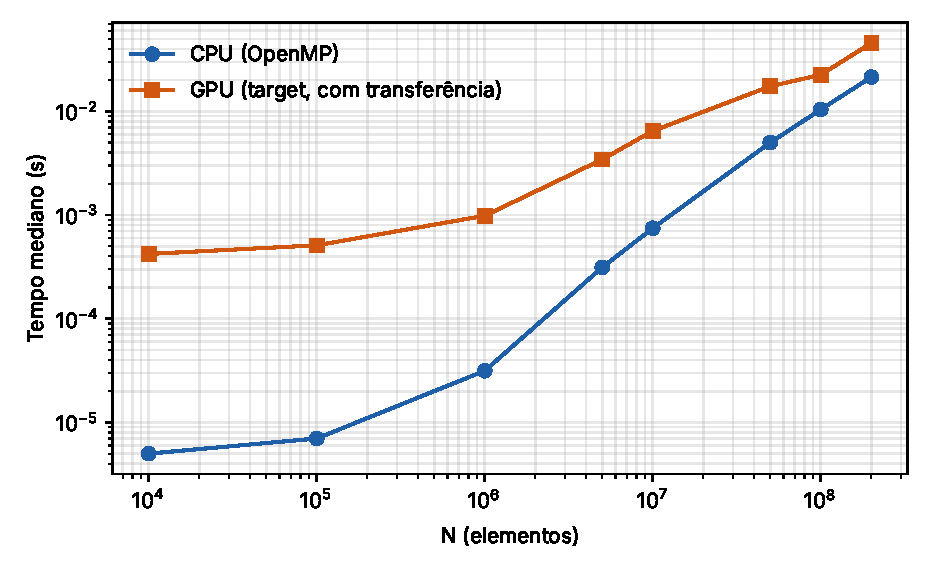
\includegraphics[width=0.8\textwidth]{../dados/grafico.pdf}
\caption{Tempo de execução em função de $N$ (escala log-log).}
\label{fig:graf}
\end{figure}

\section{Análise}

A CPU foi mais rápida que a GPU em todos os tamanhos testados. O motivo é que, nessa operação, o tempo da GPU é gasto quase todo movendo dados, não calculando:

\begin{itemize}
    \item \textbf{Pouco cálculo por dado:} cada elemento exige apenas uma soma para 12 bytes acessados. A GPU é muito rápida em cálculo, mas aqui não há cálculo suficiente para aproveitar essa vantagem.
    \item \textbf{Cópia entre CPU e GPU:} os vetores $a$ e $b$ precisam ser enviados à GPU e $c$ trazido de volta, por um barramento muito mais lento que a memória. Para $N \geq 10^8$ a vazão efetiva da GPU é de $\approx$53 GB/s, o que mostra que o tempo é o da cópia. A CPU já tem os dados na sua própria memória e não paga esse custo.
    \item \textbf{Custo fixo de lançamento:} cerca de 0,4 a 0,5 ms por chamada, mesmo com $N=10^4$. A CPU resolve esse mesmo tamanho em microssegundos.
\end{itemize}

Com o aumento de $N$ a diferença diminui (speedup de 0,01 para 0,47), pois o custo fixo passa a pesar menos, mas a GPU continua mais lenta, porque a cópia cresce junto com $N$.

\newpage
\appendix

\section{Código-Fonte}

\lstinputlisting[style=cstyle, caption={tarefa18.c}]{../src/tarefa18.c}

\end{document}